 \documentclass [12pt]{article} 

\usepackage {amsmath}
\usepackage {amsthm}
\usepackage {amssymb}
\usepackage {graphicx} 
\usepackage {float}
\usepackage {multirow}
\usepackage {xcolor}
\usepackage {algorithmic}
\usepackage [ruled,vlined,commentsnumbered,titlenotnumbered]{algorithm2e} \usepackage {array} 
\usepackage {booktabs} 
\usepackage {url} 
\usepackage {parskip} 
\usepackage [margin=1in]{geometry} 
\usepackage [T1]{fontenc} 
\usepackage {cmbright} 
\usepackage [many]{tcolorbox} 
\usepackage [colorlinks = true,
            linkcolor = blue,
            urlcolor  = blue,
            citecolor = blue,
            anchorcolor = blue]{hyperref} 
\usepackage {enumitem} 
\usepackage {xparse} 
\usepackage {verbatim}
\usepackage{listings}
\usepackage{xcolor}
\lstset { %
    language=C++,
    backgroundcolor=\color{black!5}, % set backgroundcolor
    basicstyle=\footnotesize,% basic font setting
}

\DeclareTColorBox {Solution}{}{breakable, title={Solution}} \DeclareTColorBox {Solution*}{}{breakable, title={Solution (provided)}} \DeclareTColorBox {Instruction}{}{boxrule=0pt, boxsep=0pt, left=0.5em, right=0.5em, top=0.5em, bottom=0.5em, arc=0pt, toprule=1pt, bottomrule=1pt} \DeclareDocumentCommand {\Expecting }{+m}{\textbf {[We are expecting:} #1\textbf {]}} \DeclareDocumentCommand {\Points }{m}{\textbf {(#1 pt.)}} 

\begin {document} 

{\LARGE \textbf {COMP 285 (NC A\&T, Spr `22)}\hfill \textbf {Lecture 4} } 
\vspace {1em} 
\begin {Instruction} 

Adapted From Virginia Williams' lecture notes. Additional credits: J. Su, W. Yang, Gregory Valiant, Mary Wootters, Aviad Rubinstein, Sami Alsheikh.
\end {Instruction} 

\begin{centering}
\section*{MergeSort and Introduction to Recurrence Relations}
\end{centering}

\section{MergeSort Cont.}

From last lecture, we will continue our implementation of MergeSort, and go over some of the details regarding correctness and running time.

\subsection{Correctness of MergeSort}
Let's focus on the first question first. As before, we'll proceed by induction. This time, we'll maintain a \textit{recursion invariant} that any time \texttt{MergeSort} returns, it returns a sorted array.

\begin{itemize}
    \item \textbf{Inductive Hypothesis.} Whenever \texttt{MergeSort} returns an array of size $\leq i$, that array is sorted.
    \item \textbf{Base case.} Suppose that $i = 1$. Then whenever \texttt{MergeSort} returns an array of length $0$ or length $1$, that array is sorted. (Since all array of length $0$ and $1$ are sorted). So the Inductive Hypothesis holds for $i = 1$.
    \item \textbf{Inductive step.} We need to show that if \texttt{MergeSort} always returns a sorted array on inputs of length $leq i - 1$, then it always does for length $\leq i$. Suppose that \texttt{MergeSort} has an input of length $i$. Then $L$ and $R$ are both of length $\leq i - 1$, so by induction, $L$ and $R$ are both sorted. Thus, the inductive step boils down to the statement: 

    ``When Merge takes as inputs two sorted arrays $L$ and $R$, then it returns a sorted array containing all of the elements of $L$, along with all of the elements of $R$.''

    This statement is intuitively true, although proving it rigorously takes a bit of bookkeeping. In fact, it takes another proof by induction! Check out CLRS Section 2.3.1 for a rigorous treatment.
    \item \textbf{Conclusion.} By induction, the Inductive hypothesis holds for all $i$. In particular, given an array of any length $n$, \texttt{MergeSort} returns a sorted version of that array.
\end{itemize}

\subsection{Running time of MergeSort}
Finally, we get to our first question in this lecture where the answer may not be intuitively obvious. What is the running time of \texttt{MergeSort}? In the next few lectures, we'll see a few principled ways of analyzing the runtime of a recursive algorithm. Here, we'll just go through one of the ways, which is called the \texttt{recursion tree} method.

The idea is to draw a tree representing the computation (see the slides for the visuals). Each node in the tree represents a subproblem, and its children represent the subproblems we need to solve to solve the big sub-problem. The recursion tree for \texttt{MergeSort} looks something like
this:

\begin{figure}[h!]
\centering{}
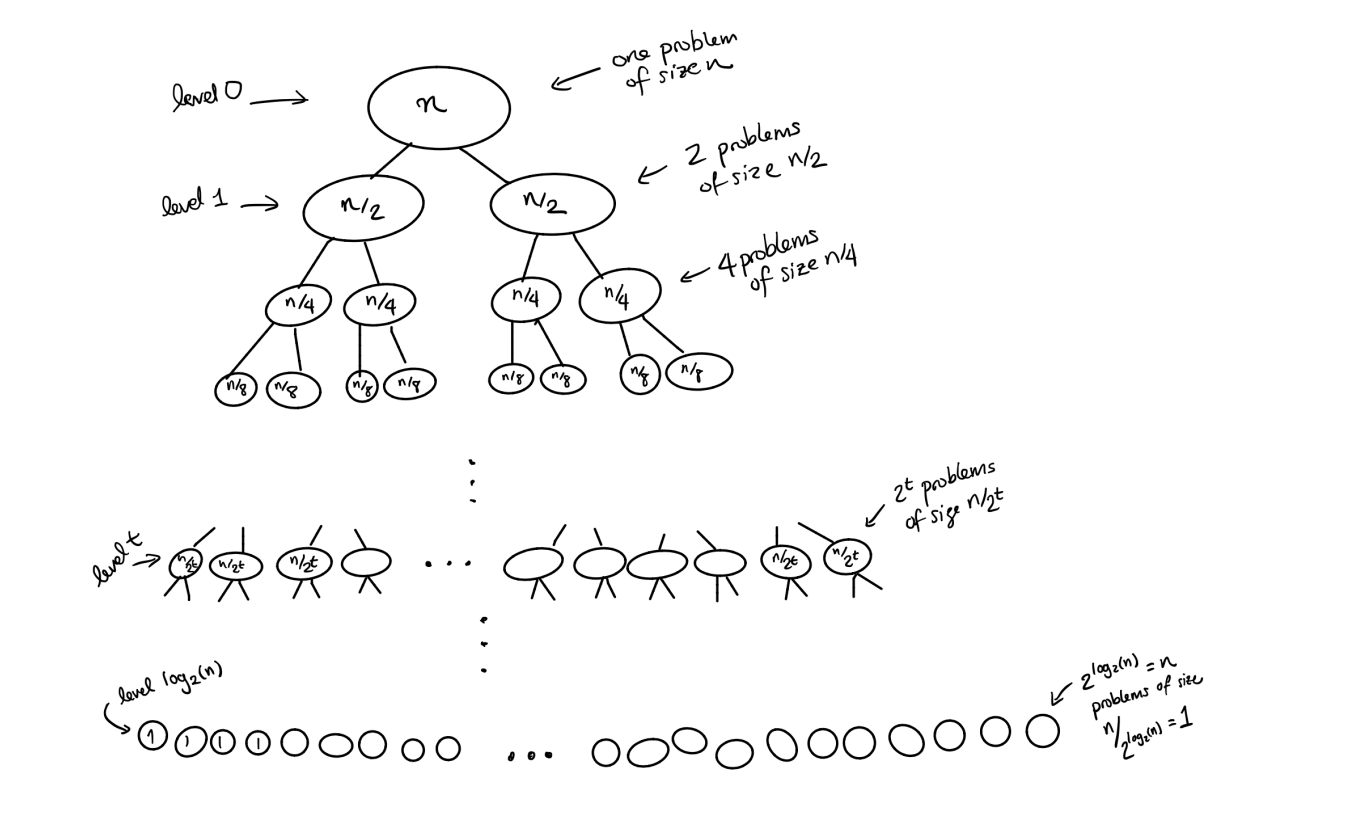
\includegraphics[scale=0.75]{mergesort_tree.png}
\end{figure}

At the top (zeroth) level is the whole problem, which has size $n$. This gets broken into two sub-problems, each of size $n/2$, and so on. At the $t$'th level, there are $2^t$ problems, each of size $n/2^t$
. This continues until we have $n$ problems of size $1$, which happens at the $log(n)$'th level.

\textbf{Some notes:}

\begin{itemize}
\item In this class, logarithms will \textbf{always} be base $2$, unless otherwise noted.
\item We are being a bit sloppy in the picture above: what if $n$ is not a power of $2$? Then $n/2^j$ might not be an integer. In the pseudocode above, we actually break a problem of size n into problems of size $\lfloor n/2 \rfloor$ and $\lceil n/2 \rceil$. Keeping track of this in our analysis will be messy, and it won't add much, so we will ignore it, and for now we will assume that $n$ is a power of $2$ \footnote{To formally justify the assumption that $n$ is a power of $2$, notice that we can always sort a \textit{longer} list of length $n' = 2^{\lceil log_2(n) \rceil}$. That is, we'll add extra entries, whose values are $\infty$, to the list. Then we sort the new list of length $n'$, and return the first $n$ values. Since $n' \leq 2n$ (why?) this won't affect the asymptotic running time. Also see CLRS Section 4.6.2 for a rigorous analysis of the original algorithm with floors and ceilings.}
\end{itemize}

In order to figure out the total amount of work, we will figure out how much work is done at each node in the tree, and add it all up. To that end, we tally up the work that is done in a particular node in the tree—that is, in a particular call to \texttt{MergeSort}. There are three things:

\begin{enumerate}
    \item Checking the base case
    \item Making recursive calls (but we don't count the work actually done in those recursive calls; that will count in other nodes)
    \item Running Merge.
\end{enumerate}

Let's analyze each of these. Suppose that our input has size $m$ (so that $m = n/2^j$ for some $j$).

\begin{enumerate}
    \item Checking the base case doesn't take much time. For concreteness, let us say that it takes one operation to retrieve the length of $A$, and other operation to compare this length to $1$, for a total of two operations.\footnote{Of course, there's no reason that the ``operation'' of getting the length of $A$ should take the same amount of time as the ``operation'' of comparing two integers. This disconnect is one of the reasons we use big-Oh notation.}
    \item Making the recursive calls should also be fast. If we implemented the pseudocode well, it should also take a constant number of operations.

        \textbf{Aside:} This is a good point to talk about how we interpret pseudocode in this class. Above, we've written \texttt{MergeSort(A[:n/2])} as an example of a recursive call. This makes it clear that we are supposed to recurse on the first half of the list, but it's not clear how we actually implement that. Our ``pseudocode'' above is in fact working Python code, and in Python, this implementation, while clear, is a bit inefficient. That is, written this way, Python will actually copy the first $n/2$ elements of the list before sending them to the recursive call. A much better way would be to instead just pass in pointers to the $0$'th and $n/2 - 1$'st index in the list. This would result in a faster algorithm, but kludgier pseudocode. In this class, we generally will opt for cleaner pseudocode, as long as it does not hurt the asymptotic running time of the algorithm. In this case, our simple-but-slower pseudocode turns out not to affect the asymptotic running time, so we'll stick with this.

    In light of the above Aside, let's suppose that this step takes $m + 2$ operations, $m/2$ to copy each half of the list over, and 2 operations to store the results. Of course, a better implementation of this step would only take a constant number (say, four) operations.
    \item The third thing is the tricky part. We claim that the Merge step also takes about $m$ operations.

    Consider a single call to Merge, where we'll assume the total size of $A$ is $m$ numbers. How long will it take for Merge to execute? To start, there are two initializations for $i$ and $j$. Then, we enter a for loop which will execute $m$ times. Each loop will require one comparison, followed by an assignment to $S$ and an increment of $i$ or $j$. Finally, we'll need to increment the counter in the for loop $k$. If we assume that each operation costs us a certain amount of time, say $Cost_a$ for assignment, $Cost_c$ for comparison, $Cost_i$ for incrementing a counter, then we can express the total time of the Merge subroutine as follows:

    $$
        2Cost_a + m(Cost_a + Cost_c + 2Cost_i)
    $$
    This is a precise, but somewhat unruly expression for the running time. In particular, it seems difficult to keep track of lots of different constants, and it isn't clear which costs will be more or less expensive (especially if we switch programming languages or machine architectures). To simplify our analysis, we choose to assume that there is some global constant $c_{op}$ which represents the cost of an operation. You may think of $c_{op}$ as $\max\{Cost_a, Cost_c , Cost_i, \dots\}$. We can then bound the amount of running time for Merge as
    $$
    2c_{op} + 4c_{op}m = 2 + 4m \text{ operations}
    $$
\end{enumerate}

Thus, the total number of operations is at most
$$
2 + (m+2) + 4m + 2 \leq 11m
$$

using the assumption that $m \geq 1$. This is a very loose bound; for larger $m$ this will be much closer to $5m$ than it is to $11m$. But, as we'll discuss more below, the difference between $5$ and $11$ won't matter too much to us, so much as the linear dependence on $m$.

Now that we understand how much work is going on in one call where the input has size $m$, let's add it all up to obtain a bound on the number of operations required for \texttt{MergeSort}. In a Merge of $m$ numbers, we want to translate this into a bound on the number of operations required for \texttt{MergeSort}. At first glance, the pessimist in you may be concerned that at each level of recursive calls, we're spawning an exponentially increasing number of copies of
\texttt{MergeSort} (because the number of calls at each depth doubles). Dual to this, the optimist in you will notice that at each level, the inputs to the problems are decreasing at an exponential rate (because the input size halves with each recursive call). Today, the optimists win out.

\textbf{Claim 3.} MergeSort \textit{requires at most $11n \log n + 11n$ operations to sort $n$ numbers}.

Before we go about proving this bound, let’s first consider whether this running time bound is good. We covered in last lecture that more obvious methods of sorting, like \texttt{InsertionSort}, required roughly $n^2$ operations. How does $n^2 = n \cdot n$ compare to $n \cdot \log n$? An intuitive definition of $\log n$ is the following: ``Enter n into your calculator. Divide by $2$ until the total is $\leq 1$. The number of times you divided is the logarithm of $n$.'' This number in general will be significantly smaller than $n$. In particular, if $n = 32$, then $\log n = 5$; if $n = 1024$, then $\log n = 10$. Already, to sort arrays of $\approx 103$ numbers, the savings of $n \log n$ as compared to $n^2$ will be orders of magnitude. At larger problem instances of $10^6, 10^9$, etc. the difference will become even more pronounced! $n \log n$ is much closer to growing linearly (with $n$) than it is to growing quadratically (with $n^2$).

One way to argue about the running time of recursive algorithms is to use recurrence relations. A recurrence relation for a running time expresses the time it takes to solve an input of size $n$ in terms of the time required to solve the recursive calls the algorithm makes. In particular, we can write the running time $T(n)$ for \texttt{MergeSort} on an array of n numbers as the following
expression.

\begin{align*}
T(n) &= T(n/2) + T(n/2) + T(Merge(n)) \\
&\leq 2\cdot T(n/2) + 11n
\end{align*}

There are a number of sophisticated and powerful techniques for solving recurrences. We will cover many of these techniques in the coming lectures. Today, we can actually analyze the running time directly.

\textit{Proof of Claim 3} Consider the recursion tree of a call to \texttt{MergeSort} on an array of $n$ numbers. Assume for simplicity that $n$ is a power of $2$. Let’s refer to the initial call as Level $0$, the proceeding recursive calls as Level $1$, and so on, numbering the level of recursion by its depth in the tree. How deep is the tree? At each level, the size of the inputs is divided in half, and there are no recursive calls when the input size is $\leq 1$ element. By our earlier ``definition'', this means the bottom level will be Level $\log n$. Thus, there will be a total of $\log n + 1$ levels.

We can now ask two questions: (1) How many subproblems are there at Level $i$? (2) How large are the individual subproblems at Level $i$? We can observe that at the $i$th level, there will be $2^i$ subproblems, each with inputs of size $n/2^i$.

We’ve already worked out that each sub-problem with input of size $n/2^
i$ takes at most $11n/2^i$ operations. Now we can add this up:

\begin{align*}
    \text{Work at Level }i &= (\text{number of subproblems}) \cdot (\text{work per subproblem}) \\
    &\leq 2^i \cdot 11 \left( \frac{n}{2^i} \right) \\
    &= 11n \text{ operations.}
\end{align*}

Importantly, we can see that the work done at Level $i$ is independent of $i - i$. It only depends on $n$ and is the same for every level. This means we can bound the total running time as follows:


\begin{align*}
    \text{Total number of operations } &= (\text{operations per level}) \cdot (\text{number of levels}) \\
    &\leq (11n)\cdot (\log n + 1) \\
    &= 11n \log n + 11n
\end{align*}
This proves the claim, and we’re done!

\section{Introduction to Recurrences}

Recall that divide and conquer algorithms divide up a problem into a number of subproblems that are the smaller instances of the same problem, solve those problems recursively, and combine the solutions to the subproblems into a solution for the original problem. When a subproblem size is small enough, the subproblem is solved in a straightforward manner. In the past lectures we have seen two examples of divide and conquer algorithms: \texttt{MergeSort} and \texttt{Karatsuba}’s algorithm for integer multiplication.

The running time of divide and conquer algorithms can be naturally expressed in terms of the running time of smaller inputs. Today we will show two techniques for solving these recurrences. The first is called the master method to solve these recurrences. This method can only be used when the size of all the subproblems is the same (as was the case in the examples).

\section{Recurrences}
Stated more technically, a divide and conquer algorithm takes an input of size $n$ and does some operations all running in $O(f (n))$ time for some $f$ and runs itself recursively on $k \geq 1$ instances of size $n_1, n_2, \dots n_k$ , where $n_i < n$ for all $i$. To talk about what the runtime of such an algorithm is, we can write a runtime \textbf{recurrence}. Recurrences are functions defined in terms of themselves with smaller arguments, as well as one or more base cases. We can
define a recurrence more formally as follows:

Let $T(n)$ be the worst-case runtime on instances of size $n$. If we have $k$ recursive calls on a given step (of sizes $n_i$) and each step takes time $O(f (n))$, then we can write the runtime as $T(n) \leq c \cdot f (n) + \sum_{i=1}^k T(n_i)$ for some constant $c$, where our base case is $T(c') \leq O(1)$.

Next lecture, we'll try to find the recurrence of some of the divide-and-conquer algorithms we've seen so far!

\end{document}